\chapter{Evaluation of integration strategies}
\label{cha:evaluation}

\section{Introduction}
\label{sec:evaluation-introduction}
In this chapter we will investigate whether different integration strategies have an impact on the performance of the resulting models. We will start of by explaining ROC analysis which is the method we use to evaluate the logistic regression models in the first case study (\ref{sec:evaluation-logisticregression}). The next section will provide details on the first case study and shows the results (\ref{sec:evaluation-predictingstage}). After that we will explain the Wald test and how we will use it to evaluate the survival models that are trained in the second case study (\ref{sec:evaluation-coxph}). The last section shows the details of the second case study and presents the results (\ref{sec:evaluation-predictingsurvival}).


\section{Evaluating a logistic regression model}
\label{sec:evaluation-logisticregression}
The first evaluation will be made using a logistic regression model. This is a model computed for a dependent variable that has a binomial distribution. To evaluate such model, a common technique used is called Receiver-Operating-Characteristic analysis~\cite{zweig1993receiver}\cite{hajian2013receiver}\cite{wikiroc} or ROC analysis for short. Remember that when we are using a logistic regression model to predict outcomes, we have to define a threshold to separate positive from negative cases. An ROC curve shows the performance of the model for any possible threshold, using metrics such as sensitivity and specificity. This gives a very good general impression of the performance of the model.
\subsection{Predictions using validation}
What we really want to do is estimate the out-of-sample error for our model. To do this we have seen that we can use the technique of cross-validation. In this case we are not going to compute any learning parameter but we are going to use the validation set as a test set. We will split our dataset into $K$ folds. We will train a model on $K-1$ folds and we will use this model to predict the outcomes of the remaining samples in the test fold. By repeating this process for each folds we obtain a predicted outcome for each sample in the dataset. Notice however that we also have the real outcome of the samples in our dataset, and thus we can compare our predictions with the real values to estimate our out-of-sample error.
\subsection{Metrics}
When we compare our models predictions with the real outcomes, there are four possible scenario's:
\begin{itemize}
	\item True Positive (TP): the model predicted positive and this is correct
	\item True Negative (TN): the model predicted negative and this is correct
	\item False Positive(FP): the model predicted positive and this is wrong (type 1 error)
	\item False Negative (FN): the model predicted negative and this is wrong (type 2 error)
\end{itemize}
Notice that this gives us more information than just registering whether we are right or wrong. It also tells us the type of mistake we made. This is a very important distinction because depending on the application there is usually a different cost attached to making type 1 or type 2 errors. And as we will see later on, there is a tradeoff between the two and we can tune our system to be more resistant towards making one type of error. \\ \\
Now that we have established the notion of typed errors, there are several ways in which these numbers are combined to form evaluation metrics. Depending on your field of research these often get different names, we will use the ones applicable to the biomedical field.
\subsubsection{Sensitivity}
Sensitivity~\cite{wikisensspec} measures the proportion of the real positive samples that our model correctly predicted as positive. It can be calculated with the following formula:
$$
Sensitivity = \frac{\sum{TP}}{\sum{P}}
$$
where
\begin{itemize}
	\item $\sum{TP}$ is the number of true positives
	\item $\sum{P}$ is the number of real positive cases in the dataset
\end{itemize}
Sensitivity can be thought of, as its name suggests, as how sensitive the model is to detecting positive cases. If the model gets a real positive sample's input, what is the probability that it will detect it as such. A sensitivity of 1 means that our model is capable of correctly identifying all positive cases in the dataset. This means that the higher the sensitivity, the lower the type 2 error rate.
\subsubsection{Specificity}
Specificity~\cite{wikisensspec} is the analogous metric to sensitivity, but for negative cases. It measures the proportion of the real negative samples that our model correctly predicts as negative.
$$
Specificity = \frac{\sum{TN}}{\sum{N}}
$$
where
\begin{itemize}
\item $\sum{TN}$ is the number of true negatives
\item $\sum{N}$ is the number of real negative cases in the dataset
\end{itemize}
A specificity of 1 means that our model is capable of correctly identifying all negative cases in the dataset. This means that the higher the specificity, the lower the type 1 error rate.
\subsubsection{The tradeoff}
At this point it is obvious that we would like to maximize both sensitivity and specificity. Indeed, if both metrics are 1 then we make no errors and we have a perfect model. In practice however this is nearly impossible to achieve. It is easy to see that there is a tradeoff between the two metrics: when we try to increase the sensitivity, we will lose out on specificity and vice versa. \\ \\ 
Consider the totally useless model that has a threshold lower than the smallest possible output. Meaning that this model will always predict a positive outcome regardless of the input. This model will have a sensitivity of 1, as we will get all positive cases correct. But it will also have a specificity of 0 because we get none of the negative cases correct. As we gradually increase the threshold we will cross critical values where some sample inputs will now produce an output below the threshold and thus be classified as negatives. If this happens to be a correct prediction our specificity will go up and sensitivity will remain unchanged. If it happens to be an error, specificity is unchanged and sensitivity will go down. The gradual increase of the threshold will thus cause sensitivity to drop and specificity to increase, up to the point where we reach the other extreme. The threshold is now bigger than the biggest possible output and the model always predicts negative regardless of the input. This threshold gives us a sensitivity of 0 and a specificity of 1.
\subsection{Receiver Operating Characteristic curve}
The ROC curve is a way of showing exactly this gradual increase of the threshold. The typical way of constructing a ROC curve is to put $(1-specificity)$ on the X-axis and $sensitivity$ on the Y axis. The values for these metrics are then plotted for values of the threshold ranging from the all-positive model to the all-negative model. An example ROC curve is shown on figure \ref{fig:evaluation-roc}. The metric we will use to evaluate the performance of different models is the area under the ROC curve (AUC). This metric works because it indicates how far we can optimize both sensitivity and specificity for different thresholds. It shows how close we can get to the upper left corner of the plot, which indicates the perfect model. The AUC metric ranges from 0 to 1, but in fact its value is only informative in between 0.5 and 1. Imagine a model that makes completely random predictions, this model will get a correct prediction 50\% of the time. If we would create a ROC curve for this model we would on average get a straight diagonal line from the bottom left to the top right. This line is therefore considered a lower bound for the performance of a model.
\begin{figure}
	\centering
	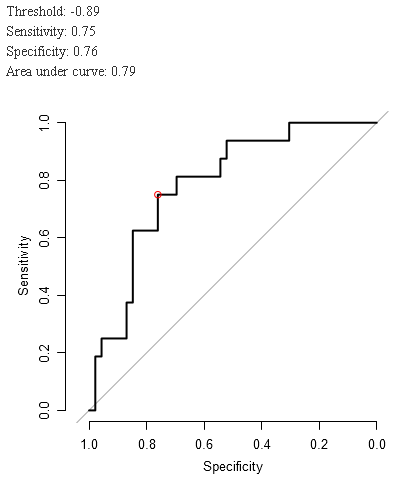
\includegraphics[scale=.9]{images/roc_curve}
	\caption{Example ROC curve and metrics}
	\label{fig:evaluation-roc}
\end{figure}
\section{Case study 1: predicting stage outcome}
\label{sec:evaluation-predictingstage}
\subsection{Case details}
\label{sec:evaluation-casedetails}
The case we are showing here uses datasets created by the University Hospital of Leuven in a study on colorectal cancer patients. There are three source datasets that all contain imaging data: a dataset from MRI (Magnetic Resonance Imaging) scans, a dataset from DWI (Diffusion Weighted Magnetic Resonance Imaging) scans, and a dataset from PET (Positron Emission Tomography) scans. It is important to note that these scans were taken three times per patient at different periods in their treatment: one in the beginning, one roughly in the middle, and one near the end. This means that there is some temporal information present in the datasets, but this has been encoded in the explanatory variables. For instance: there is a variable in the MRI dataset that shows the size change of the tumour between the first and second scan. In this way we can treat this as a regular explanatory variable and we don't have to worry about the temporal aspect. \\ \\
The dependent variable is a binary outcome based on whether the patient got a pathologically complete response. For a more in-depth explanation on what this means see appendix \ref{app:cancer-staging}. For now, we can view a positive outcome as a patient who has recovered from the cancer, and a negative outcome as a patient that has not. The aim is now to build a model that receives the explanatory variables from the scans as input, and predicts the outcome for that patient.
\subsection{The results}
The resulting AUC's for the individual and integrated datasets are shown respectively in tables \ref{tab:evaluation-auc-individual} and \ref{tab:evaluation-auc-integrated}. We can clearly see that the model for the individual MRI dataset contains the most predictive information out of the three datasets. This however doesn't mean that the other datasets are useless. Indeed, when we integrate the other dataset with the MRI dataset we get even better performances. From table \ref{tab:evaluation-auc-integrated} we can see that in this case the intermediate integration method outperforms the other strategies regardless of which datasets are used. \\ \\
We have also included an overview of the model parameters that were selected (on average) by each strategy. The values in this table show the weights given to each corresponding variable in the model. A positive weight indicates that a higher value for this variable increases the chance of a positive outcome. A negative weight correlates the variable with a decreased probability of positive outcome. The overview is shown in table \ref{tab:evaluation-model-parameters}. The first column shows the name of the selected variable, these are imaging features. The next three columns show the model parameters for the individual models. The last two columns show the parameters that were selected by the integrated models. It is interesting to see how all models tend to select the same kind of variables and give them similar weights. This shows us that these variables indeed do contain some predictive information. Notice that the intermediate model selects fewer variables than the other models, while still outperforming them. It removes those variables that have very small weights in other models and thus acts as a very strict variable selector. This is no surprise if we remember how the intermediate integration method uses two steps of variable selection to perform the integration (chapter \ref{cha:integration}, section \ref{sec:integration-intermediate}).

\begin{table}
	\centering
	\begin{tabular}{lc}
		\toprule
		Dataset & AUC \\
		\midrule
		DWI & 0.67 \\
		MRI & 0.75 \\
		SUV & 0.65 \\
		\bottomrule
	\end{tabular}
	\caption{Area under the ROC curve for models of individual datasets}
	\label{tab:evaluation-auc-individual}
\end{table}
\begin{table}
	\centering
	\begin{tabular}{lcccc}
		\toprule
	 & All & DWI+MRI & DWI+SUV & MRI+SUV \\
		\midrule
		Early integration & 0.76 & 0.82 & 0.69 & 0.74 \\
		Intermediate integration & 0.79 & 0.83 & 0.78 & 0.75 \\
		Late integration & 0.73 & 0.78 & 0.66 & 0.70 \\
		\bottomrule
	\end{tabular}
	\caption{Area under the ROC curve for models of various combinations of integrated datasets}
	\label{tab:evaluation-auc-integrated}
\end{table}


\begin{table}
	\rowcolors{1}{white}{lightgray}
	\centering
	\begin{tabular}{lccccccc} 
		\toprule
		\multicolumn{1}{c}{}& \multicolumn{3}{c}{Individual} & \multicolumn{2}{c}{}&  \multicolumn{2}{c}{Integrated}\\ 
		\cmidrule{2-8}
		Variable & DWI    & MRI & SUV & & & Early    & Intermediate\\ 
		\midrule
		ADCratioavg\_TP1TP3 		& 0.69	& 		&  		& & & 1.09		& 1.19	\\ 
		ADCratiohigh\_TP1TP3 		& 0.08	&      	&  		& & & 0.50		& 0.62	\\ [10pt]
		DeltaSphere\_TP2TP3perc 	&      	& 1.67  &  		& & & 1.35		& 1.44  \\
		DeltaSphere\_TP1TP3perc 	&      	& 0.48  &  		& & & 1.78		& 1.64  \\
		Volume\_TP2 				&  		& -0.99 &   	& & & 			& 		\\
		Volume\_TP3 				&  		& -0.24 &   	& & & -0.173	& -0.94	\\ [10pt]
		RIdiameter\_TP2TP3 			&  		&      	& 0.16  & & & 			& 		\\
		Diameter\_TP3 				&  		&      	& -0.88 & & & -0.01		& 		\\
		SUVmax\_TP2 				&  		&      	& -0.88 & & & -3.30		& -4.41	\\
		deltadiameter\_TP1TP2 		&  		&      	& -0.32 & & & 			& 		\\
		RISUVpeak\_TP1TP2 			&  		&      	&  		& & & 0.32		& 		\\
		RITLG\_TP2TP3 				&  		&      	&  		& & & -0.08		& 		\\
		\bottomrule
	\end{tabular}
	\caption{Overview of the model parameters (weights) for all of the computed models}
	\label{tab:evaluation-model-parameters}
\end{table}

\section{Evaluating a cox proportional hazards model}
\label{sec:evaluation-coxph}
The evaluation of a cox proportional hazards model is different compared to logistic regression~\cite{newson2010comparing}\cite{harrell1996tutorial}. This is because, as we have seen in chapter \ref{cha:cox}, we normally don't directly compute survival times from a cox proportional hazards model. This means we cannot compare them to the real survival times. However we can still evaluate the models based on statistics that indicate significance.

\subsection{Predictions for survival models}
Recall the hazard ratio from section \ref{sec:cox-proportional-hazards-model}. If we have a model computed ($\beta's$ defined) and we have a test sample (with values $X_{i}$ for the explanatory variables), we could compute the following prediction quantity:
\begin{equation}
\begin{split}
prediction = exp(\sum_{i=0}^{N}X_{i}\beta_{i})
\end{split}
\end{equation}
where
\begin{itemize}
	\item $exp(x)$ is the exponential of x
	\item $X_{i}$ are the values for the explanatory variables
	\item $\beta_{i}$ are the model coefficients
\end{itemize}
 We can view this as the hazard ratio between the test sample and an imaginary patient that has the value $0$ for all explanatory variables which we will call the baseline patient (subscript $b$):
 \begin{equation}
 \begin{split}
 \frac{\lambda_{i}(t)}{\lambda_{b}(t)} 
 = \frac{\lambda_{0}(t)e^{X_{i1}\beta_{1} + ... + X_{iN}\beta_{N}}}{\lambda_{0}(t)e^{0\beta_{1} + ... + 0\beta_{N}}}
 = e^{(X_{i1}-0)\beta_{1} + ... + (X_{iN}-0)\beta_{N}} = exp(\sum_{j=0}^{N}X_{ij}\beta_{j})
 \end{split}
 \end{equation}
 What this quantity tells us is whether the risk of our test patient is higher or lower than the risk of the baseline patient. This does not tell us anything in the absolute sense about survival times, but we can compare this prediction value in a relative way between patients. \\ \\
 We could, as we did in section \ref{sec:evaluation-logisticregression}, compute this prediction value for all patients in our dataset using cross-validation. We now want to test the predictive value of these predictions. To do this we construct a new survival model, but this time there is only one explanatory variable and that is our vector of predictions. If we can show that this variable is significant in predicting the survival, then our original model is also significant. The significance test we will use is called the Wald Test.
 
 \subsection{The Wald test}
 \label{subsec:evaluation-wald-test}
The Wald test~\cite{wikiwald} is a statistical test that can be used to test the significance of an estimated parameter. The Wald test can be used on a single parameter or on a vector of parameters at once. In the case of one parameter $\beta$ the formula for the Wald test is:
\begin{equation}
\begin{split}
\frac{(\hat{\beta}-\beta_{0})^{2}}{var(\hat{\beta})} \sim \tilde{\chi}^{2}_{1}
\end{split}
\end{equation}
where
\begin{itemize}
	\item $\hat{\beta}$ is the maximum likelihood estimate we calculated and want to test
	\item $\beta_{0}$ is the value of $\beta$ if the null-hypothesis is true
	\item $var(\beta)$ is the variance of $\beta$
	\item $\tilde{\chi}^{2}_{1}$ is the chi-squared distribution with one degree of freedom
\end{itemize}
When we are testing the significance of a coefficient in our survival model we have to compare it against a so called null-hypothesis. In this case the null-hypothesis is the model where all coefficients are equal to zero. The values for $\hat{\beta}$ and $var(\beta)$ are defined by the model. Intuitively the Wald test computes the distance between the obtained value for the parameter and the parameter value under the null-hypothesis, relative to the variance of the parameter. If the variance is large, then we are unsure about the value for the parameter that we calculated and it is harder to reject the null-hypothesis. An example is demonstrated on figure \ref{fig:evaluation-wald-test}. \\ \\
\begin{figure}
	\centering
	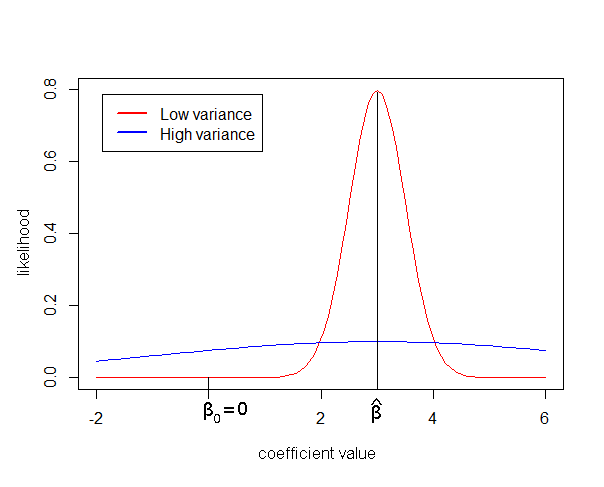
\includegraphics[scale=.7]{images/wald_test}
	\caption{Example Wald test variance visualisation. Both curves give the same maximum likelihood estimate $\hat{\beta}$. The red curve however has low variance, providing good evidence to reject the null-hypothesis with value $\beta_{0}$. The blue curve has high variance, in this case $\hat{\beta}$ does not significantly differ from $\beta_{0}$ and we cannot reject the null-hypothesis.}
	\label{fig:evaluation-wald-test}
\end{figure}
The Wald test can tell us something about the significance of the predictions vector and therefore about the predictive ability of our initial model. We can go one step further and compute a p-value~\cite{pvalue1}\cite{wikip} for the wald-test statistic. This p-value contains the exact same information as the wald-test statistic, but it is a very well known quantity statistics so we will add it for completeness.
\section{Case study 2: predicting survival outcomes}
\label{sec:evaluation-predictingsurvival}

\subsection{Case details}
\label{sec:evaluation-casedetails2}
The case we are showing here uses datasets from The Cancer Genome Atlas~\cite{tcga}. TCGA is a 2.5 petabyte database of cancer data for 33 different types of cancer made publicly available for research. We will only use a subset of this database for this case study. The cancer type we will use is called Colon adenocarcinoma, or COAD for short. From this cancer we will use 3 datasets: the first contains copy number variation (CNV) data. CNV's indicate the deletions or duplications of parts of DNA causing there to be more (or less) copies of this piece of DNA. The second dataset contains information about the messenger RNA (mRNA) which directly influences the expression of genes. The last dataset contains information about micro RNA (miRNA) which is known to have an RNA silencing function and also regulates gene expression. This last dataset is extra interesting because there is already evidence that abnormal expression of miRNA is correlated with cancer development\cite{iorio2005microrna}\cite{yanaihara2006unique}\cite{wikimicrorna}. The dependent variables in this case are survival data, and as we have seen in chapter \ref{cha:cox} this involves a time vector and a censoring vector. \\ \\
Table \ref{tab:evaluation-case2-dimensions} presents the dimensions of the used datasets. It is worth mentioning that these datasets are all the result of a preprocessing step to make them ready for analysis. However the preprocessing is not the main focus of this thesis so we will not go into any more detail.
\begin{table}
	\centering
	\begin{tabular}{lcc}
		\toprule
		Dataset name & Number of variables & Number of patients \\
		\midrule
		Copy Number Variations & 16 & 219\\
		messenger RNA & 3869 & 219 \\
		micro RNA & 414 & 219 \\
		\bottomrule
	\end{tabular}
	\caption{Dimensions for the datasets used in the survival analysis.}
	\label{tab:evaluation-case2-dimensions}
\end{table}
\subsection{The results}
The resulting performance statistics for all the models are shown in tables \ref{tab:evaluation-surv-individual} and \ref{tab:evaluation-surv-integrated}. The first table shows the statistics for the models of individual datasets. The second table shows the statistics for the integrated datasets.
\subsection{Interpretation of the statistics}
The first statistic is the hazard ratio. This number shows the multiplicative effect on the hazard for a unit increase of the variable. Remember from section \ref{sec:evaluation-predictingsurvival} that the variable in this case is the vector of predictions. The predictions are the result of our originally trained model. A hazard ratio of 1.39 thus means that a unit increase in the outcome of the model has the effect of increasing the hazard by 39\%. \\ \\
The second statistic is the hazard ratio confidence interval. This shows the lower and upper bounds of the 95\% confidence interval for the hazard ratio. If this interval is very wide then this means the value for the hazard ratio is uncertain. The narrower the interval, the more certain we are about the predicted value for the hazard ratio. \\ \\
The third statistic is the wald test, which has been explained in section \ref{subsec:evaluation-wald-test}. The larger this number, the more significant the results of that model are. This is immediately related to the fourth, and last, statistic which is the p-value for the wald test. This value also indicates the significance of the model that we have obtained. A usual practice in statistics is to say that an observation (or model in this case) is significant if the p-value is below the 0.05 threshold.
\subsection{Interpretation of the results}
It is immediately clear that the majority of the models are not significant. The p-values are way too high, the wald test scores are too low, and the confidence intervals are too wide to say anything meaningful about the obtained hazard ratios. However it is interesting to note that all the integrated models have a significantly lower p-value when compared to the individual models. In fact, the intermediate integrated model actually reaches a p-value that is lower than the threshold of 0.05 which makes this model significant. More research would have to be performed if one really wanted to use this model to make predictions, but for our purposes this analysis is sufficient to conclude that the integrated models have outperformed the individual models and they clearly have an impact on the performance of the resulting model.
\begin{table}
	\centering
	\begin{tabular}{lccc}
		\toprule
		 & CNV    & mRNA & miRNA \\
		\midrule
		Hazard ratio (HR) 			& 1.39	& 0.74	& 0.84	\\
		HR Confidence interval 		& [0.29 - 6.72]	& [0.14 - 3.87]	& [0.64 - 1.11] \\
		Wald test 					& 0.17 & 0.13  & 1.46 \\
		P-value 					& 0.6799 & 0.7209  & 0.2276 \\
		\bottomrule
	\end{tabular}
	\caption{Performance statistics for survival models of individual datasets}
	\label{tab:evaluation-surv-individual}
\end{table}

\begin{table}
	\centering
	\begin{tabular}{lccc} 
		\toprule
		& Early & Intermediate & Late\\
		\midrule
		Hazard ratio (HR) 			& 0.96	& 0.90 & 0.13	\\
		HR Confidence interval 		& [0.03 - 1.47]	& [0.82 - 1.00] & [0.01 - 2.24]	\\
		Wald test 					& 2.43 & 3.89 & 1.98 \\
		P-value 					& 0.1192 & 0.0485 & 0.1595 \\
		\bottomrule
	\end{tabular}
	\caption{Performance statistics for integrated survival models}
	\label{tab:evaluation-surv-integrated}
\end{table}

\section{Conclusion}
\label{sec:evaluation-conclusion}
In this chapter we have shown the results of the two case studies that we performed. The first section (\ref{sec:evaluation-logisticregression}) explains how we use ROC analysis to evaluate the logistic regression models that resulted from the first case study. The results of this case study (section (\ref{sec:evaluation-predictingstage})) show that indeed the intermediate integration strategy outperforms all other strategies aswell as the individual models, which provides evidence for the thesis aim that integration strategies have an impact on the performance of the resulting models. The third section ((\ref{sec:evaluation-coxph})) explains how we come up with predictive values in a survival analysis and how we can use the wald test to evaluate the significance of the obtained models. The last section ((\ref{sec:evaluation-predictingsurvival})) shows the results of the second case study on survival data obtained from TCGA. The results of this study are less evident than those of the first case study due to insignificance of most of the models. But we can still conclude that the integration strategies had an impact on the performance of the models.
%%% Local Variables: 
%%% mode: latex
%%% TeX-master: "thesis"
%%% End: 
